\documentclass[twocolumn]{article}
\usepackage{datetime}
\usepackage{hyperref}
\usepackage{listings}
\usepackage{color}
\usepackage{graphicx}

\begin{document}

% Source code highlighting
\definecolor{javared}{rgb}{0.6,0,0} % for strings
\definecolor{javagreen}{rgb}{0.25,0.5,0.35} % comments
\definecolor{javapurple}{rgb}{0.5,0,0.35} % keywords
\definecolor{javadocblue}{rgb}{0.25,0.35,0.75} % javadoc
\lstset{language=Java,
	basicstyle=\ttfamily\tiny,
	keywordstyle=\color{javapurple}\bfseries,
	stringstyle=\color{javared},
	commentstyle=\color{javagreen},
	morecomment=[s][\color{javadocblue}]{/**}{*/},
	numbers=none,
	stepnumber=2,
	numbersep=10pt,
	tabsize=2,
	showspaces=false,
showstringspaces=false,
framesep=0pt}

% Title
\pagenumbering{gobble}
\begin{titlepage}


\vspace*{15em}


\centering

{\LARGE
Department of Electrical \& Computer Engineering \\
Final Year Research Project 2015, Interim Report}

\hspace{2em}

% notes on latex tables use "&" as colum sperator
\begin{table*}[h]
\centering
\begin{tabular}{ll}
Project Title: & Preventing plagiarism during practical tests \\
Project Number: & 11 \\
Supervisor Name: & Dr Nasser Giacaman \\
Second Examiner Name: & Avinash Malik \\
Your Name: & Kurt McAlpine \\
Your UID: & 2004750 \\
Partner Name: & Conor Simmonds \\
Date submitted: & 11\textsuperscript{th} May 2015 \\

\end{tabular}
\end{table*}
\begin{table}


\end{table}
\pagebreak

\vspace*{25em}

{\Large Declaration of Originality}

\hspace{5em}

This report is my own unaided work and was not copied from 
nor written in collaboration with any other person.

Name: Kurt McAlpine


\end{titlepage}



\pagenumbering{arabic}

\begin{abstract}

Software engineering courses today have impractical test environments. They are
performed using pen and paper, without access to a computer, compiler, IDE or
the internet. Active Test Programmer gives the students the opportunity to be
tested in a practical manner and gives the teacher confidence that plagiarism
will be caught. Practical tests will give students a more realistic assessment
of their abilities in the real world. Practical tests also give industry
recruiters more confidence that students that graduate from such programmes have
good practical skills. 

\end{abstract}

\section{Introduction}
In the world today, programming and programs are prevalent and abundant in our
every day lives. Therefore it is an important skill. It's
widely accepted that programming is a difficult skill to learn
\cite{jenkins2002difficulty, robins2003learning}. There is a need to innovate
and devise solutions to help students be more effective in class.
When students struggle in class with tests and assignments, it can lead to
plagiarism or even dropping out\cite{bennedsen2007failure}. Currently in many
institutions, software engineering courses test their students on their
knowledge and skill in a way that is artificial to real world programming.
For example, tests are done with pen and paper and without access to computers with
IDE`s, compilers or the internet. Therefore, in this project we want to construct a
way to give software engineering students robust testing environments that allow
students to have a more realistic set of tools during the test. However, whilst
giving students these tools we would also like to give the teaching staff
confidence that plagiarism can be detected automatically without tedious manual
inspection of student submissions as well as detecting plagiarised work that the
student has attempted to conceal.
% TODO overview of report

\section{Background}
Eclipse is an IDE (Integrated Development Environment) that is written in Java.
It can be used to develop in a variety of programming languages. It also has
a plugin architecture which allows other developers to extend its functionality
without changing its core implementation.

There are several plagiarism detection tools available for institutions to use.
Two of which are MOSS\cite{schleimer2003winnowing} and
JPlag\cite{lutz2000jplag}. Both these systems are utilised on submissions from
students to help identify any similarities between the students' work. If the student
submissions are too similar, these tools will detect that and warn the lecturer
that plagiarism is the likely cause of this similarity.

A tool called ACP (Active Classroom Programmer)\cite{giacaman2015active} is used
at the University of Auckland in SOFTENG 701 and 751. ACP is an eclipse
plugin that allows the lecturer to create eclipse workspaces and upload
snapshots of the current state to a web server. For example during a lecture a
task can be completed in parts and once each part is complete a snapshot of the
code can be uploaded. The students, during the lecture can download these
snapshots using the ACP eclipse plugin, onto their laptops and make
modifications and experiment with the workspace, they can also attempt to
complete the next part before the lecturer has completed it. Often there are
short breaks during the lecture that allow students to attempt the tasks.

Active Test Programmer (ATP) is an extension to ACP which allows the lecturer to
setup a programming test. The programming test can be distributed to students
before the test starts. The test is encrypted so a secret code is needed to
decrypt the tests. When a secret code is distributed to the students they may
type it in and begin the test. After a predetermined amount of time the the test
is over and the students must submit their code through the eclipse plugin.

\section{Active Test Programmer}
For my project, we are going to extend ATP to give lecturers confidence that
plagiarism that has occurred during the test can be detected automatically. The
way this will be done is the history of the student completing the test will be
recorded and when the test is submitted the history will go with it. This
history gives us much richer insight into the characteristics of the students
work. Analysis of the history of the students submission will allow for more
robust detection of potential plagiarism.

\subsection{Features} \label{sec:Features}
Create tests: The lecturer will be able to create a programming test in their
IDE and upload it. Once the test is uploaded the lecturer will be given a secret
code that can be used to begin the test.

Download tests: Students will be able to download tests from within their IDE,
they may not begin the test until they have entered the secret code to decrypt
the test. This allows all the students to download and be ready for the test, so
that everyone may begin at the same time, and no students will feel
disadvantaged because it took them longer to download the test, or if WiFi is
unavailable the test may be distributed on a USB flash drive.

Upload completed test: Students may upload their completed test through their
IDE. If WiFi is unavailable they may export their completed test to an archived
file and copy it to a flash drive to give to the lecturer. The archived
completed test will contain information about when it was exported so that we
can be sure they completed the test in the given time.

Implementation history: The completed test that the student uploads, will
contain a complete history in snapshots over time of how the test was
implemented. This gives a rich insight into potential plagiarism in the history
of the code.

Viewing reports: Reports can be generated that contain analyses of student
tests. In the analyses it will contain a score of how likely it was that the
students submission contains plagiarised work. The history also gives us the
opportunity to go beyond just checking for plagiarism.

\section{Technologies Considered}
For this project the client application will be implemented using the Eclipse
plugin framework. There are other IDE's that could potentially be used because
it also have a plugin architecture for example IntelliJ but Eclipse was chosen
because ACP is already implemented for Eclipse and it's going to be extended to
contain the features outlined in \nameref{sec:Features}.

For recording the history of the changes to files in the students test, libgit2
will be used. libgit2 can be used to store the history of a file in a series of
commits. The reason libgit2 will be used is that is has a permissive license so
it can be integrated into this project without license concerns. Implementing a
system of storing changes to a file isn't feasible for a small project like this
so libgit2 is a good fit.

\section{Implementation}

I have implemented several components that make up the software solution for my
project. First is the Eclipse Plugin which is an end user oriented plugin
available for students to install onto their machines. Code Report Tool is a
command line application used for the analysis of individual test submissions.
Finally Code Analysis Tool is used in conjunction with Code Report Tool to
aggregate information retrieved from multiple student test submissions.

\subsection{Eclipse Plugin}

\begin{figure}[h!]
\centering
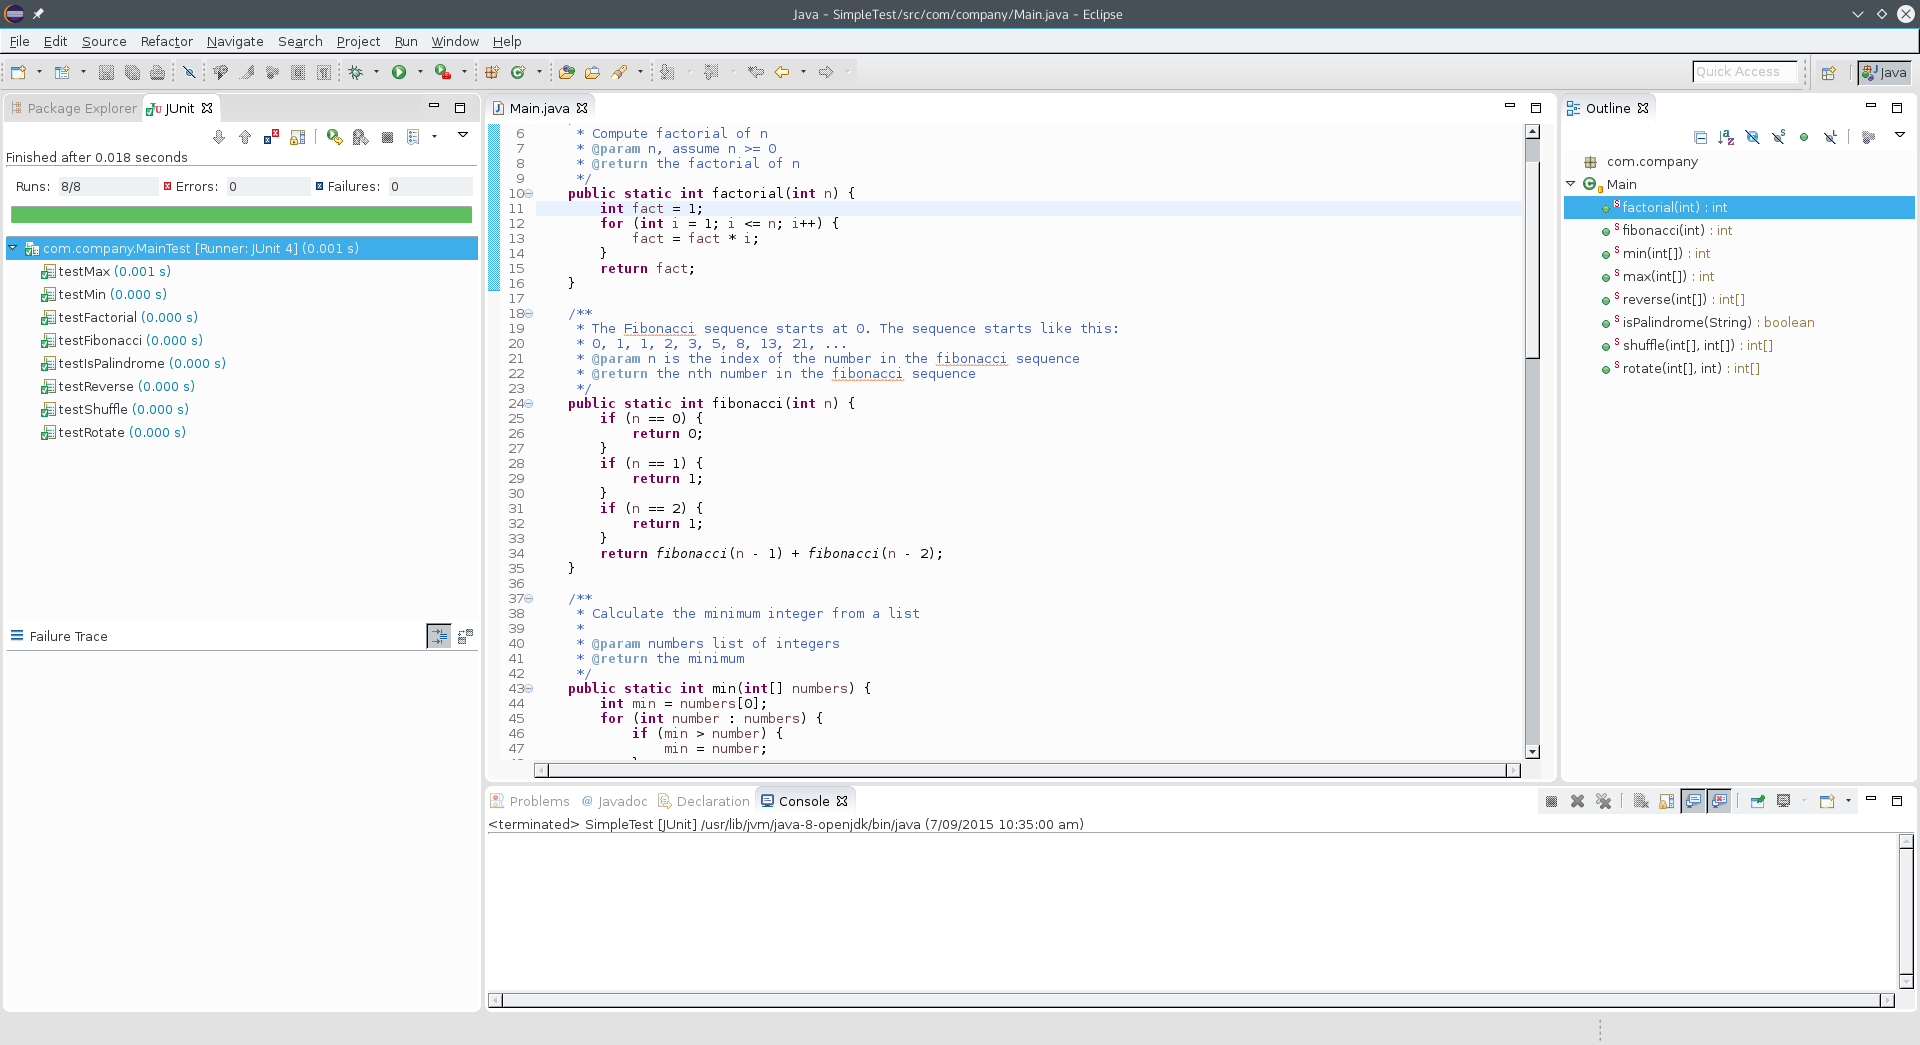
\includegraphics[width=\linewidth]{figures/eclipse}
\caption{Screenshot of a test in progress}
\end{figure}

Eclipse was the IDE of choice for this project due to its use in undergraduate
classes at the University of Auckland. The plugin I have developed for Eclipse
allows us to give students a test as an Eclipse project. Students can copy this
test from the internet for via USB drive or other portable storage device
handed out by the instructor. During the test the plugin keeps track of what
the user is doing and records a fair amount of information to the local data
storage device. When the test is complete the student must submit the Eclipse
project to the instructor so that we may do some analysis as well as grade the
test.\\

Whilst the student is using Eclipse during a test with the plugin installed.
The plugin is able to attach an event listener to current document objects. The
document object represents the text editor in Eclipse used to modify code. The
event listener is able to listen to keystroke and view focus events. What is
happening under the hood whist the student modifies code during the test is
that the plugin saves the current edited document to the local storage device
every time at least one second has passed and an event is fired. This limits
the maximum frequency of writes to local storage device to be exactly one per
second. This frequency may be adjusted if needed by from my experience with an
old inexpensive laptop from 2012, there is no noticeable performance hit with a
frequency of one per second. In addition to writing the file to local storage
at a maximum frequency of once per second a Git commit is created. A Git commit
is essentially a snapshot of the current state of all the files in the project.
The use of Git as a snapshot file format is a very convenient way to store the
data. The Git interface is simple so it allowed me to quickly develop a way to
save snapshots of a file. It is space efficient as it only stores file
differences and not copies of files. The interface also allows use to easily
retrieve a snapshot from any point in time which is convenient for when we want
to analyse snapshots of a students test submission.\\

When the student submits their project all the history comes along with the
project stored in a directory named \texttt{.git}. Which we may use to perform
our analysis.

\subsection{Code Report Tool}

Code Report Tool is a tool that I developed to attempt to simplify extraction
data from the students test submissions. It provide an interface for traversing
history of a test submission and extracting certain data.\\

An example of the series of snapshots that can be retrieved from a repository
are shown below. The following are snapshots from a test that I completed, all
the snapshots are able to be parsed by the Java compiler.
\begin{lstlisting}[frame=single]
public static int max(int[] numbers) {
	return 	0;
}
\end{lstlisting}
\begin{lstlisting}[frame=single]
public static int max(int[] numbers) {
	int max = numbers[0];
	return 	0;
}
\end{lstlisting}
\begin{lstlisting}[frame=single]
public static int max(int[] numbers) {
	int max = numbers[0];
	for (int i = 0; i < numbers.length; i++) {
	}
	return 	0;
}
\end{lstlisting}
\begin{lstlisting}[frame=single]
public static int max(int[] numbers) {
	int max = numbers[0];
	for (int i = 0; i < numbers.length; i++) {
		if (max < numbers[i]) {
		}
	}
	return 	0;
}
\end{lstlisting}
\begin{lstlisting}[frame=single]
public static int max(int[] numbers) {
	int max = numbers[0];
	for (int i = 0; i < numbers.length; i++) {
		if (max < numbers[i]) {
			max = numbers[i];
		}
	}
	return 	0;
}
\end{lstlisting}
\begin{lstlisting}[frame=single]
public static int max(int[] numbers) {
	int max = numbers[0];
	for (int i = 0; i < numbers.length; i++) {
		if (max < numbers[i]) {
			max = numbers[i];
		}
	}
	return 	max;
}
\end{lstlisting}

What Code Report Tools allows us to do is point it to a submitted test and
extract some simple metrics. Since we have a first snapshot and a final
snapshot we can calculate the length of time spent working on the test. This
measurement is more accurate than comparing the submission time to the start
time as there are many factors that could delay the start of a test as well as
delays which would cause the student submit the test after he or she has
completed the test. Using the snapshots we can accurately determine precisely
when they started modifying the test to when they stop modifying the test.

Since we can calculate the length of time spent working on the test, we can
also calculate the average characters per minute. Since we have a snapshot for
every state of the test we can count the amount of characters added to the test
and then get the average typing speed.

A more sophisticated analysis may be performed if instead of analysing only the
textual snapshots, we analyse the abstract syntax trees that can be built from
the repository of snapshots. An abstract syntax tree or AST is a representation
of the source code in the form of a tree that allows us to perform a deeper
analysis.

An example of abstract syntax trees build for different snapshots are shown in
figures \ref{fig:ast1}, \ref{fig:ast2}, \ref{fig:ast3} and \ref{fig:ast4}. In
figure \ref{fig:ast1} we see a file \texttt{Main.java} which contains the class
\texttt{Main} which contains several methods. This may be the initial state
before the student has modified any methods. In the next figure (figure
\ref{fig:ast2}) we see a variable \texttt{n} has been declared in the method
\texttt{factorial}. In figure \ref{fig:ast3} we see an ``if block'' has been added
to \texttt{factorial}. And finally in figure \ref{fig:ast4} another variable
\texttt{x} has been declared in the ``if block''.

\begin{figure}[h!bt]
\centering
\includegraphics[width=\linewidth]{figures/ast/ast1}
\caption{Initial AST}
\label{fig:ast1}
\centering
\includegraphics[width=\linewidth]{figures/ast/ast2}
\caption{Variable declaration node added to method node}
\label{fig:ast2}
\centering
\includegraphics[width=\linewidth]{figures/ast/ast3}
\caption{If block added to method node}
\label{fig:ast3}
\centering
\includegraphics[width=\linewidth]{figures/ast/ast4}
\caption{Variable declaration node added to method node}
\label{fig:ast4}
\end{figure}

These AST snapshots can be automatically generated by Code Report Tool. And an
analysis example has been implemented inside Code Report Tool to calculate the
time spend modifying each method. We can calculate the time spent modifying
each method by building the AST for every possible snapshot and then comparing
those AST's in chronological order to see which nodes have been modified.
Taking into account the time stamps for those snapshots we can determine how
much time was spent modifying a method.

\subsection{Code Analysis Tool}
The final tool that I have implemented I have unimaginatively named Code
Analysis Tool. What it does is gives the instructor a user interface to collect
data from test submissions. The user of this tool provides a path to the
directory of student test submissions and runs the analyses of their choosing.
The output is graphed data so that the instructor may use this information to
make choices about what their focus should be in classes. Examples of this are
shown in figures \ref{fig:test_len}, \ref{fig:chars} and \ref{fig:method_time}.

\begin{figure}[h!bt]
\centering
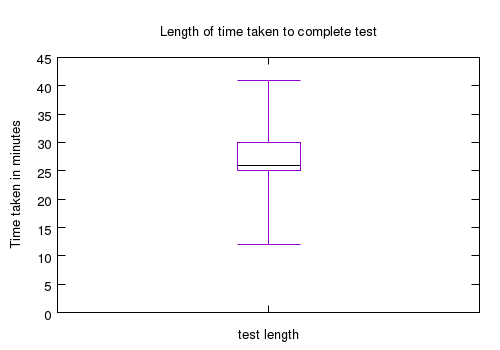
\includegraphics[width=\linewidth]{figures/test_length}
\caption{Distribution of time taken to complete the test}
\label{fig:test_len}
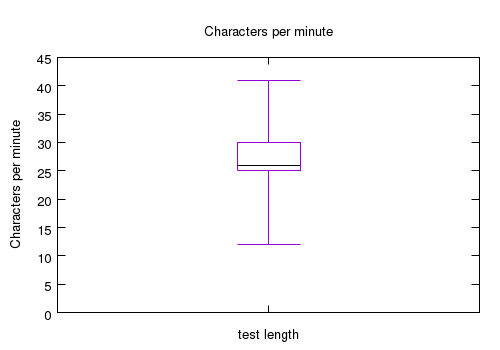
\includegraphics[width=\linewidth]{figures/char_per_minute}
\caption{Distribution of character per minute}
\label{fig:chars}
\end{figure}

In figure \ref{fig:method_time} note how \texttt{isPalindrome} took on average
the longest to implement by all the students. This side by side plot of method
implementation times may help the instructor to determine which topics the
class is struggling the most and he or she may be able to tailor the course
content to compensate for that.

\begin{figure}[h!bt]
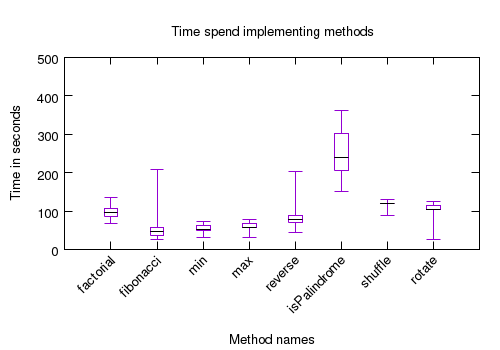
\includegraphics[width=\linewidth]{figures/method_time}
\caption{Distribution of time spent implementing methods}
\label{fig:method_time}
\end{figure}

Analysis of a single students performance is also possible. In figure
\ref{fig:student1} a red line shows how a chosen student performed in
comparison to the distribution. Note that this particular student accounts for
the maximum in the distribution for implementing the method
\texttt{isPalindrome}, this may be an indication to the instructor to talk to
this student about course content covered by that particular method
implementation.

\begin{figure}[h!bt]
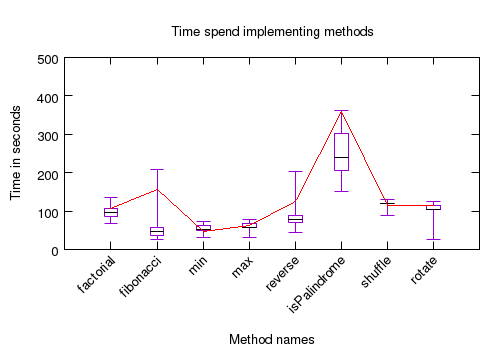
\includegraphics[width=\linewidth]{figures/student1}
\caption{Individual student shown in red}
\label{fig:student1}
\end{figure}

It is also possible to compare two students. Shown in figure \ref{fig:student2}
two students are being compared, one in greed the other in red.

\begin{figure}[h!bt]
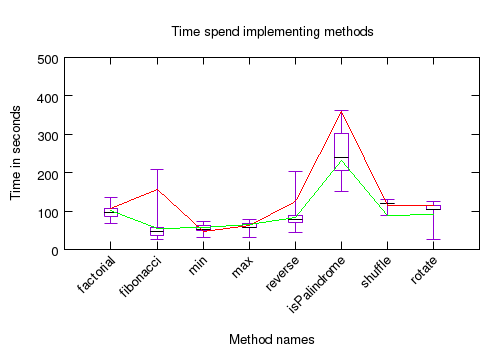
\includegraphics[width=\linewidth]{figures/student2}
\caption{Comparing two students one in green one in red}
\label{fig:student2}
\end{figure}

\subsection{Open Source Tools}
All the tools I have developed for this project are licensed under the GNU
General Public Licence and are available for free from \url{github.com}. As
well as the source code there are instructions for building and using the tools
and they are available here:
{\footnotesize
\begin{itemize}
\item \url{https://github.com/kurtmc/EclipseHistoryPlugin}
\item \url{https://github.com/kurtmc/CodeReportTool}
\item \url{https://github.com/kurtmc/CodeAnalysisTool}
\end{itemize}
}


\section{Evaluation}
Unfortunately due to time constraints and issues arising from implementation no
evaluation has been performed. Evaluation is important for convincing an
audience that it is a worthwhile investment. In the future it may be possible
to distribute the tools that I have implement and field test them. Since all
the tools are publicly available it may be possible for someone interested to
use them in a real life setting.

\section{Future Work}
Given more time and more development resources I would like to have seen more
things implemented. One useful tool that should have been implemented is a web
service that allows students to be delivered the test within the IDE, and once
the test is completed submit the test from within the IDE. This web service
would also allow the instructor to download all the tests and perform the
analyses of his or her choosing.

Furthermore I would like to have implemented plugins not only for Eclipse.
Eclipse is not the only IDE used for Java development and it would be silly to
claim realistic testing environments when we have to restrict which IDE
students may use. Eclipse is also a major limitation as whilst working on this
project Eclipse released a new version of their IDE which makes changed to the
plugin architecture which breaks the plugin I have developed. So currently the
only version of Eclipse that can be used with my plugin is Eclipse Luna and not
Eclipse Mars.


\section{Conclusions}
Since the focus of this project has changed from one interested in avoiding
plagiarism to one that generalises the analyses that can be performed during
practical programming tests. I think the tools I have implemented are a
starting point that can be extended into a suite of testing analysis tools that
can give course instructors insight into the performance of their students that
was not possible with the classical pen and paper tests.

\bibliographystyle{IEEEtran}
\bibliography{references}

\end{document}
